
In the last three Chapters we have introduced six important \PETSc types (object classes).  All are important for solving PDEs:

\medskip
\begin{tabular}{ll}
Chapter \ref{chap:ls}: \pVec, \pMat, \pKSP, \pPC \hspace{.5in} & for linear algebra \\
Chapter \ref{chap:st}: \pDMDA                    & for structured grids \\
Chapter \ref{chap:nl}: \pSNES                    & for Newton's method
\end{tabular}

\bigskip

Each example in the rest of the book will use \pVec, \pMat, \pKSP, \pPC, and \pSNES.  From now on we will even solve linear PDEs using a \pSNES object, for example in Chapter \ref{chap:ad}.  In such cases we know that one Newton iteration suffices in theory.  Always using \pSNES allows uniform code structure and more flexibility when it comes to changing the PDE problem.

Though new ideas appear in it, the current Chapter takes a break from introducing new \PETSc types.  Instead we look at a PDE which arises from minimization in a function space, and we introduce a structured-grid finite element method.  This example is a nonlinear Poisson-like equation with solution-dependent diffusivity.

The example code here is the last one shown in full.  In later Chapters we show snippets.  The reader can always examine and run the complete codes by looking in the \texttt{c/} directory of the \texttt{p4pdes} repository; see Chapter \ref{chap:gs}.


\section{$p$-Laplacian equation as minimization}

Let $\Omega$ be a domain (connected open subset) in $\RR^2$ with well-behaved boundary.\sidenote{A Lipschitz boundary will suffice in theory.  In practice we use polygonal domains, namely a rectangle in the current Chapter and general polygons in Chapter \ref{chap:un}.}  For simplicity, noting our numerical method will use the point values of this function, suppose $f\in C(\overline \Omega)$ is given.  Consider this nonliner functional for $p \ge 1$,
\begin{equation}
    I[u] = \int_\Omega \frac{1}{p} |\grad u|^p - fu.  \label{eq:of:functional}
\end{equation}
It is well-defined and continuous on the Sobolev space \citep{AdamsFournier2003,Evans2010} of integrable functions on $\Omega$ which have integrable gradient,
\begin{equation}
    W^{1,p}(\Omega) = \left\{w \,:\, \int_\Omega |w|^p < \infty \,\, \& \, \int_\Omega |\grad w|^p < \infty\right\}. \label{eq:of:sobolevdefn}
\end{equation}
This is a Banach space with norm $\|w\|_{W^{1,p}} = \left(\int_\Omega |w|^p + \int_\Omega |\grad w|^p\right)^{1/p}$.

\begin{marginfigure}
\includegraphics[width=1.2\textwidth]{figs/minsurf} % generated by figs/minsurf.tex
\medskip
\caption{The functional $I[u]$ is analogous to the convex surface $z = \tfrac{1}{4}(x^4 + y^4) - 2x + 2y$ shown here, but with input from the $\infty$-dimensional space $W_g^{1,p}(\Omega)$ instead of the plane $\RR^2$.}
\label{fig:of:cartoonfunctional}
\end{marginfigure}

The reader may visualize $I[u]$ in cartoon form as in Figure \ref{fig:of:cartoonfunctional}.  As suggested by the cartoon, this functional has a unique minimum, at least once we add boundary conditions.  We add Dirichlet conditions (Chapter \ref{chap:st}) by choosing a real-valued function $g$, defined along $\partial \Omega$, so as to determine an affine subspace of $W^{1,p}(\Omega)$, namely
\begin{equation}
    W_g^{1,p}(\Omega) = \left\{w \,:\, w \in W^{1,p}(\Omega) \,\, \& \,\, w\big|_{\partial \Omega} = g\right\}.  \label{eq:of:affinedirichlet}
\end{equation}
For this to make sense one might require $g \in L^p(\partial \Omega)$ and note that the equation $w\big|_{\partial \Omega} = g$ has a precise ``trace operator'' meaning \citep[section 5.5]{Evans2010}.  Again, however, because our numerical scheme will use the point values of $g$, we assume $g\in C(\partial\Omega)$.

The above considerations also define the vector subspace $W_0^{1,p}(\Omega) \subset W^{1,p}(\Omega)$ in the case where $g=0$.  We will use this subspace for ``test functions'' below.

The functional $I[u]$ has two significant properties.  First, $I[u]$ is \emph{coercive} in the sense that if the input function from $W_g^{1,p}(\Omega)$ is large in norm then the output is large:
\begin{equation}
\lim_{\|u\|_{W^{1,p}} \to +\infty} I[u] = +\infty.   \label{eq:of:coercivity}
\end{equation}
Second it is \emph{convex}, meaning that
\begin{equation}
I[\lambda u + (1-\lambda) v] \le \lambda I[u] + (1-\lambda) I[v]    \label{eq:of:convexity}
\end{equation}
if $u,v\in W_g^{1,p}(\Omega)$ and $0 \le \lambda \le 1$.  (We say inequality \eqref{eq:of:convexity} is \emph{strict} if $\|u-v\|_{W^{1,p}} > 0$ and $0 < \lambda < 1$.)
These two properties of $I[u]$, coercivity and convexity, are addressed in Exercise \ref{chap:of}.\ref{exer:of:twoproperties}.

A standard theorem in the calculus of variations \citep[Theorem 8.2.2]{Evans2010} shows that the coercivity and strict convexity of $I[u]$ imply that the problem
\begin{equation}
\min_{u \in W_g^{1,p}(\Omega)} I[u] \label{eq:of:plapmin}
\end{equation}
has a unique solution.  Strict convexity is used to show uniqueness, but convexity also implies that $I[u]$ is continuous enough to have a minimum on compact sets in the appropriate topology.\sidenote{Namely $I[u]$ is \emph{weakly lower semi-continuous}. This means, by definition, that $\liminf_{v\rightharpoonup u} I[v] \ge I[u]$, using the weak topology on $W^{1,p}(\Omega)$ \citep[section 8.2]{Evans2010}.}  Compactness arises from coercivity in the sense that bounded, closed subsets of $W^{1,p}(\Omega)$, which arise in the existence proof as sets $\{w\,:\,I[w] \le L\}$, are compact in the weak topology.

Being good calculus students we seek the solution to minimization problem \eqref{eq:of:plapmin} by taking the derivative and setting it to zero.  If $p>1$ then the functional $I[u]$ is smooth enough to have a gradient, as we show next.  The solution of minimization \eqref{eq:of:plapmin} is then also the solution to a nonlinear equation.  It has several names, including \emph{variational equation}, \emph{Euler-Lagrange equation}, and the \emph{weak form of the PDE}.

Assume $\eps\in \RR$ and $u,v \in W^{1,p}(\Omega)$.  Then, by the binomial theorem,
\begin{align*}
I[u+\eps v] - I[u] &= \int_\Omega \frac{1}{p} |\grad u + \eps \grad v|^p - \frac{1}{p} |\grad u|^p - \eps f v \\
   &= \eps \left(\int_\Omega |\grad u|^{p-2} \grad u \cdot \grad v - f v\right) + O(\eps^2).
\end{align*}
Thus the directional derivative exists and has this formula:
\begin{equation}
\grad I[u](v) = \lim_{\eps\to 0} \frac{I[u+\eps v] - I[u]}{\eps} = \int_\Omega |\grad u|^{p-2} \grad u \cdot \grad v - f v. \label{eq:of:plapfunctionalderivative}
\end{equation}
That is, for each $u \in W^{1,p}(\Omega)$, formula \eqref{eq:of:plapfunctionalderivative} defines a linear and continuous map, the gradient
   $$\grad I[u] : W^{1,p}(\Omega) \to \RR.$$

If $u \in W_g^{1,p}(\Omega)$ and $v\in W_0^{1,p}(\Omega)$ then $u+\eps v\in W_g^{1,p}(\Omega)$.  Thus if $u \in W_g^{1,p}(\Omega)$ solves \eqref{eq:of:plapmin} then the above calculation also shows $\grad I[u](v)=0$ or
\begin{equation}
\int_\Omega |\grad u|^{p-2} \grad u \cdot \grad v - f v = 0 \label{eq:of:plapweakform}
\end{equation}
for all $v\in W_0^{1,p}(\Omega)$.  Note that the test functions $v$ have zero boundary values in this calculation.  We refer to \eqref{eq:of:plapweakform} as the \emph{weak form} of the $p$-\emph{Laplacian} equation.

If the solution $u \in W_g^{1,p}(\Omega)$ to minimization problem \eqref{eq:of:plapmin} or equation \eqref{eq:of:plapweakform} is actually smooth enough to have continuous second derivatives\sidenote{\emph{Proving} this much smoothness is possible in some cases when the domain $\Omega$ and data $f,g$ are well-behaved, but beyond our scope.} then we can derive the \emph{strong form} PDE as follows.  An integration-by-parts \citep[Appendix C]{Evans2010} gives
    $$-\int_\Omega \Div\left(|\grad u|^{p-2} \grad u\right) v - \int_\Omega f v + \int_{\partial \Omega} v |\grad u|^{p-2} \grad u \cdot \bn = 0.$$
The boundary integral is zero because $v\in W_0^{1,p}(\Omega)$.  It follows that
\begin{equation}
- \Div\left(|\grad u|^{p-2} \grad u\right) = f.
\label{eq:of:plapstrongform}
\end{equation}
This strong form is the traditional form of the $p$-Laplacian equation.  It reduces to the Poisson equation \eqref{poissonsquare} if $p=2$.

Before proceeding to a numerical solution, the main ideas of the above diversion into theory are simple and worth restating:
\begin{quote}
Minimization problem \eqref{eq:of:plapmin} is equivalent to the weak form \eqref{eq:of:plapweakform}.  These become the strong form \eqref{eq:of:plapstrongform} when the solution $u$ is smooth.  Thus the $p$-Laplacian equation, either \eqref{eq:of:plapweakform} or \eqref{eq:of:plapstrongform}, arises from minimization.
\end{quote}


\section{Structured $Q^1$ finite elements}

Initially, we can use \PETSc to numerically solve the $p$-Laplacian equation as minimization problem \eqref{eq:of:plapmin}, based only on user code that computes the functional $I[u]$ from a representation of $u \in W_g^{1,p}(\Omega)$.  Thus, once we have a finite-dimensional representation of the input $u$, we need to implement formula \eqref{eq:of:functional} for $I[u]$.

Such a minimization approach may suffice for prototyping.  It can then be augmented by additional derivative-computing code so that the problem becomes a nonlinear-residual problem like that of Chapter \ref{chap:nl}.  Initially, however, we will ask \PETSc to use finite differences when it needs derivatives (gradients) in minimizing $I[u]$.  In this case the nonlinear equations, and the associated residual functions, are only approximate and are internal to \PETSc.

For the representation of $u$ we introduce a structured-grid finite element method (FEM) using quadrilateral elements.  The gridded unknowns, which live on a structured grid somewhat different from that in Chapter \ref{chap:st}, now represent a function in a function space.  The resulting code will be similar to a finite difference solution of PDE \eqref{eq:of:plapstrongform}, despite the conceptual changes.

\begin{figure}
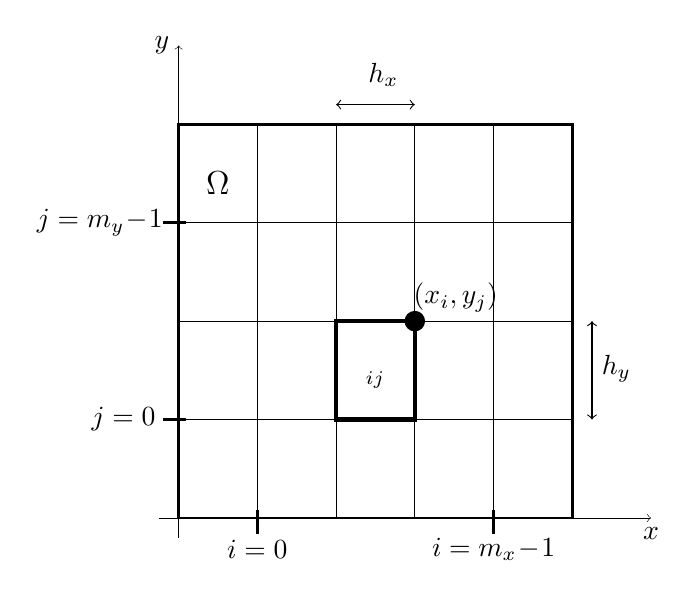
\begin{tikzpicture}[scale=5.0]
  % axes
  \draw[->,very thin] (-0.05,0.0) -- (1.2,0.0) node[below] {$x$};
  \draw[->,very thin] (0.0,-0.05) -- (0.0,1.2) node[left] {$y$};
  % grid
  \draw[line width=1.0pt] (0.0,0.0) -- (0.0,1.0) -- (1.0,1.0) -- (1.0,0.0) -- cycle;
  \pgfmathsetmacro\fifth{1.0/5.0}
  \pgfmathsetmacro\fourth{1.0/4.0}
  \draw[xstep=\fifth,ystep=\fourth,black,thin] (0.0,0.0) grid (1.0,1.0);
  \node at (0.1,0.85) {\large $\Omega$};
  % outline an element, showing location and dimensions
  \draw[line width=1.5pt] (0.6,0.5) -- (0.4,0.5) -- (0.4,0.25) -- (0.6,0.25) -- cycle;
  \node at (0.5,0.35) {$\square_{ij}$};
  \filldraw (0.6,0.5) circle (0.7pt) node[xshift=5.2mm,yshift=3mm] {$(x_i,y_j)$};
  \draw[<->] (0.4,1.05) -- (0.6,1.05) node[above,yshift=1mm,xshift=-4mm] {$h_x$};
  \draw[<->] (1.05,0.25) -- (1.05,0.5) node[right,yshift=-6mm] {$h_y$};
  % tick marks for i
  \draw[line width=1.0pt] (0.2,-0.04) -- (0.2,0.02);
  \draw[line width=1.0pt] (0.8,-0.04) -- (0.8,0.02);
  \node[yshift=-4mm] at (0.2,0.0) {$i=0$};
  \node[yshift=-4mm] at (0.8,0.0) {$i=m_x\!-\!1$};
  % tick marks for j
  \draw[line width=1.0pt] (-0.04,0.25) -- (0.02,0.25);
  \draw[line width=1.0pt] (-0.04,0.75) -- (0.02,0.75);
  \node[xshift=-7mm] at (0.0,0.25) {$j=0$};
  \node[xshift=-10mm] at (0.0,0.75) {$j=m_y\!-\!1$};
\end{tikzpicture}
\medskip

\caption{The structured grid divides the unit square $\Omega$ into elements $\square_{ij}$ of area $h_x h_y$.  There are $m_x\times m_y$ interior nodes (degrees of freedom).  We index elements by their upper-right corners $(x_i,y_j)$.}
\label{fig:of:q1grid}
\end{figure}

The domain used in this Chapter is the square $\Omega = (0,1)\times (0,1)$.  Consider the structured grid on $\Omega$ shown in Figure \ref{fig:of:q1grid}.  In this structured grid, only \emph{interior} nodes represent unknowns, because the boundary values of $u\in W_g^{1,p}(\Omega)$ are known from $g$.

Let $m_x,m_y$ be positive integers and define $h_x = 1/(m_x+1)$ and $h_y = 1/(m_y+1)$.  Define a structured grid:
\begin{equation}
x_i = (i+1) h_x, \qquad y_j = (j+1) h_y. \label{eq:of:structuredgridindexing}
\end{equation}
These formulas apply for $i=-1,0,\dots,m_x$ and $j=-1,0,\dots,m_y$, giving $\tilde N = (m_x+2)(m_y+2)$ total nodes in the grid, but the $N=m_x\, m_y$ interior nodes are points with $0 \le i \le m_x-1$ and $0 \le j \le m_y-1$.  The interior nodes correspond to the degrees of freedom.  The grid has $(m_x+1)(m_x+1)$ rectangular \emph{elements}
   $$\square_{ij} = [x_{i-1},x_i] \times [y_{j-1},y_j]$$
for $i=0,\dots,m_x$ and $j=0,\dots,m_y$.  We index the elements by their upper-right node (corner).  Each element has area $|\square_{ij}| = h_x h_y$.

The functional in \eqref{eq:of:functional} can be computed element-by-element,\footnote{Because element boundaries have zero measure and integration is additive.}
\begin{equation}
I[u] = \sum_{i=0}^{m_x} \sum_{j=0}^{m_y} \int_{\square_{ij}} \frac{1}{p} |\grad u|^p - fu  \label{eq:of:sumoverelements}
\end{equation}
Integration over a single element $\square_{ij}$ can be addressed once we represent $f$ and $u$.  A similar sum over elements computes an approximation of the weak form \eqref{eq:of:plapweakform}; see (5.FIXME).

How should we approximate a function $w \in W^{1,p}(\Omega)$ in a manner compatible with a structured grid of rectangles?  One simple choice requires that the approximation $w_h$ be bilinear on each element $\square_{ij}$ and continuous on the whole domain $\Omega$.  These requirements determine $w_h(x,y)$ from the nodal values $w_{ij} = w_h(x_i,y_j)$.  Said another way, there is a linear isomorphism between the vector space $\RR^{\tilde N}$, and an $\tilde N$-dimensional linear subspace of $W^{1,p}(\Omega)$, namely
\begin{equation}
S^h = \left\{v \in C(\Omega) \, \Big| \, v|_{\square_{ij}} \text{ is bilinear}\right\}. \label{eq:of:Shdefn}
\end{equation}
Because the elements are quadrilaterals and the degree of bilinear polynomials is one, $S^h$ is a $Q^1$ \emph{finite element space} \citep{Elmanetal2005}

The solution $u$ to minimization problem \eqref{eq:of:plapmin} must, however, have the boundary values given by $g$.  We require $g$ to be continuous and (appropriately) piece-wise linear on $\partial\Omega$, as otherwise its use conflicts with the restrictions which define $S^h$.  One may then show that the functions
\begin{equation}
S_g^h = \left\{v \in S^h \, \Big| \, v|_{\partial \Omega} = g\right\} \label{eq:of:Sghdefn}
\end{equation}
form an (affine) subspace of $W_g^{1,p}(\Omega)$.  Replacing $W_g^{1,p}(\Omega)$ by $S_g^h$ in problem \eqref{eq:of:plapmin} is a \emph{conforming}\sidenote{A ``nonconforming'' version might have $u_h|_{\partial \Omega}$ as the piecewise-linear interpolant of $g$.} $Q^1$ FEM.  Because an element of $S_g^h$ is entirely determined by its values on interior nodes, so $S_g^h$ is an $N=m_x m_y$ dimensional affine subspace of $S^h$.

The next step is to describe a bilinear function on a single element $\square_{ij}$, and to thereby build a basis for space $S_g^h$.  We do this by constructing bilinear functions on a \emph{reference element}
    $$\square_\ast = [-1,1]\times[-1,1]$$
in variables $\xi$ and $\eta$, as shown in Figure \ref{fig:of:q1gridandref}.\sidenote{One may easily avoid using the reference element because all elements are congruent rectangles.  We are, however, thinking ahead toward unstructured examples (Chapter \ref{chap:un}).}

If $v(\xi,\eta)$ is bilinear on $\square_\ast$ then $v(\xi,\eta) = a + b\, \xi + c\, \eta + d\, \xi \eta$.  The monomial basis $\{1,\xi,\eta,\xi\eta\}$ is not, however, a convenient one.  Instead, number the vertices (nodes) of $\square_\ast$ as shown in Figure \ref{fig:of:q1gridandref}:
\begin{align}
(\xi_0,\eta_0) &= (+1,+1), \quad (\xi_1,\eta_1) = (-1,+1),    \label{eq:of:refcorners} \\
(\xi_2,\eta_2) &= (-1,-1), \quad (\xi_3,\eta_3) = (+1,-1). \notag
\end{align}
The four functions
\begin{equation}
\chi_\ell(\xi,\eta) = \frac{1}{4} \left(1 + \xi_\ell \xi\right) \left(1 + \eta_\ell \eta\right)  \quad \text{ for } \ell=0,1,2,3 \label{eq:of:chidefn}
\end{equation}
form a basis of bilinear functions on $\square_\ast$.  The nodal values satisfy $\chi_\ell(\xi_{\ell'},\eta_{\ell'}) = \delta_{\ell\ell'}$ so expanding in this basis uses coefficients equal to the nodal values:
\begin{equation}
v(\xi,\eta) = \sum_{\ell=0}^3 v(\xi_\ell,\eta_\ell) \chi_\ell(\xi,\eta). \label{eq:of:bilinearrepresentationref}
\end{equation}

\begin{figure}
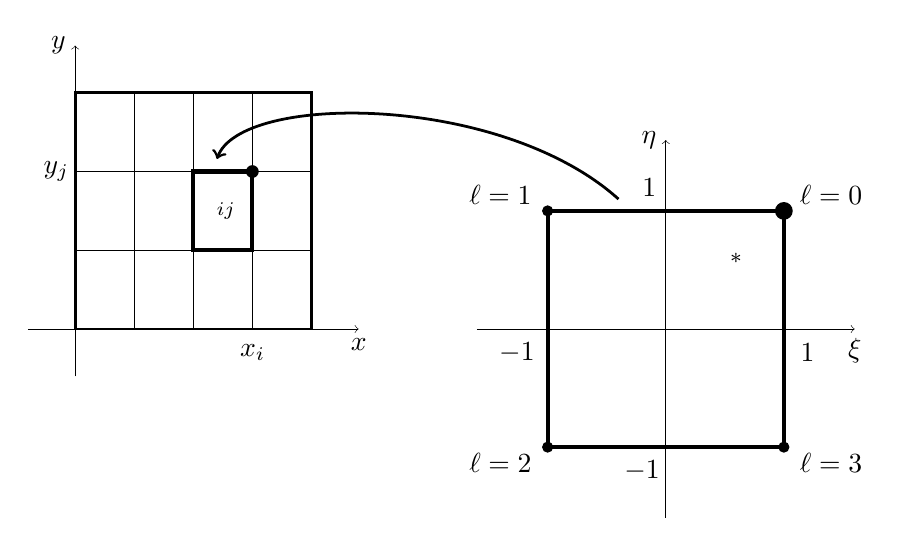
\begin{tikzpicture}[scale=3.0]
% (x,y) elements
  \draw[->,very thin] (-0.2,0.0) -- (1.2,0.0) node[below] {$x$};
  \draw[->,very thin] (0.0,-0.2) -- (0.0,1.2) node[left] {$y$};
  \draw[line width=1.0pt] (0.0,0.0) -- (0.0,1.0) -- (1.0,1.0) -- (1.0,0.0) -- cycle;
  \pgfmathsetmacro\fourth{1.0/4.0}
  \pgfmathsetmacro\third{1.0/3.0}
  \pgfmathsetmacro\twothird{2.0/3.0}
  \draw[xstep=\fourth,ystep=\third,black,thin] (0.0,0.0) grid (1.0,1.0);
  % outline an element
  \draw[line width=1.5pt] (0.5,\third) -- (0.75,\third) -- (0.75,\twothird) -- (0.5,\twothird) -- cycle;
  \node at (0.64,0.5) {$\square_{ij}$};
  \node at (0.751,-0.1) {$x_i$};
  \node at (-0.08,\twothird) {$y_j$};
  \filldraw (0.75,\twothird) circle (0.7pt);

% (xi,eta) reference element
% origin of axes at (2.5,0.0) and square has half-width 0.5
  \draw[->,very thin] (1.7,0.0) -- (3.3,0.0) node[below] {$\xi$};
  \draw[->,very thin] (2.5,-0.8) -- (2.5,0.8) node[left] {$\eta$};
  \draw[line width=1.5pt] (2.0,-0.5) -- (3.0,-0.5) -- (3.0,0.5) -- (2.0,0.5) -- cycle;
  \node at (3.1,-0.1) {$1$};
  \node at (1.87,-0.1) {$-1$};
  \node at (2.43,0.6) {$1$};
  \node at (2.4,-0.6) {$-1$};
  \node at (2.8,0.3) {\large $\square_\ast$};
  \filldraw (3.0,0.5) circle (1.0pt) node[xshift=6mm,yshift=2mm] {$\ell=0$};
  \filldraw (2.0,0.5) circle (0.6pt) node[xshift=-6mm,yshift=2mm] {$\ell=1$};
  \filldraw (2.0,-0.5) circle (0.6pt) node[xshift=-6mm,yshift=-2mm] {$\ell=2$};
  \filldraw (3.0,-0.5) circle (0.6pt) node[xshift=6mm,yshift=-2mm] {$\ell=3$};
% arc:
  \draw[->,line width=1.0pt] (2.3,0.55) .. controls (1.8,1.0) and (0.7,1.0) .. (0.6,0.72);
\end{tikzpicture}
\caption{Each element $\square_{ij}$ is the image under a map from the reference element $\square_\ast$.  The corners of $\square_\ast$ are numbered $\ell=0,1,2,3$.  The $\ell=0$ corner maps to $(x_i,y_j)$.}
\label{fig:of:q1gridandref}
\end{figure}

The element map $\square_\ast \to \square_{ij}$ pictured in Figure \ref{fig:of:q1gridandref} can be written using the above basis functions $\chi_\ell$, or in simplified form:
\begin{align}
x(\xi,\eta) &= \sum_{\ell=0}^3 x_\ell \chi_\ell(\xi,\eta) = x_i + \frac{h_x}{2} (\xi-1), \label{eq:of:referencemap} \\
y(\xi,\eta) &= \sum_{\ell=0}^3 y_\ell \chi_\ell(\xi,\eta) = y_j + \frac{h_y}{2} (\eta-1). \notag
\end{align}
The Jacobian of this map, used in integrals below, is the ratio of the area of $\square_{ij}$ to that of $\square_\ast$:
\begin{equation}
\det\frac{\partial(x,y)}{\partial(\xi,\eta)} = \det\begin{bmatrix} \frac{h_x}{2} & 0 \\ 0 & \frac{h_y}{2} \end{bmatrix} = \frac{h_x h_y}{4}. \label{eq:of:elementjacobian}
\end{equation}

\begin{marginfigure}
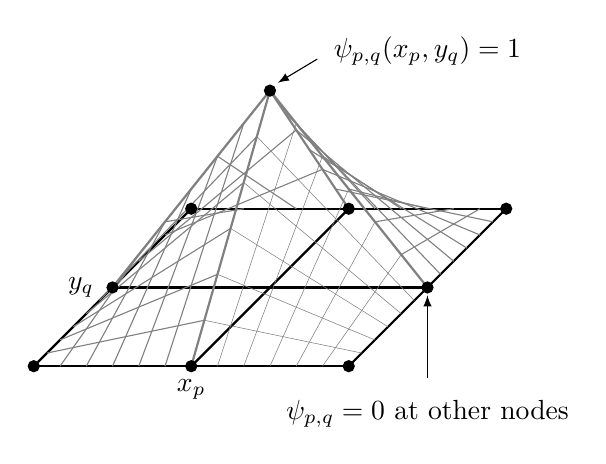
\begin{tikzpicture}[scale=0.5]

  % strong grid around elements
  \draw[thick] (0,0) -- (8,0);
  \draw[thick] (2,2) -- (10,2);
  \draw[thick] (4,4) -- (12,4);
  \draw[thick] (0,0) -- (4,4);
  \draw[thick] (4,0) -- (8,4);
  \draw[thick] (8,0) -- (12,4);

  \def\ytop{7};

  % tent lines
  \draw[gray,thick] (6,\ytop) -- (4,0);
  \draw[gray,thick] (6,\ytop) -- (2,2);
  \draw[gray,thick] (6,\ytop) -- (10,2);
  \draw[gray,thick] (6,\ytop) -- (8,4);

  \def\dx{(10.0-6.0)/6};
  \def\dy{(2.0-\ytop)/6};
  \foreach \jj in {1,...,5}
  {
       \draw[gray,very thin] ({6+\jj*\dx},{\ytop+\jj*\dy}) -- ({4+(4/6)*\jj},0.0);
  }

  \def\dx{(4.0-6.0)/6};
  \def\dy{(0.0-\ytop)/6};
  \foreach \jj in {1,...,5}
  {
       \draw[gray,very thin] ({6+\jj*\dx},{\ytop+\jj*\dy}) -- ({10-(2/6)*\jj},{2-(2/6)*\jj});
  }

  \def\dx{(2.0-6.0)/6};
  \def\dy{(2.0-\ytop)/6};
  \foreach \jj in {1,...,5}
  {
       \draw[gray,thin] ({6+\jj*\dx},{\ytop+\jj*\dy}) -- ({4-(4/6)*\jj},0.0);
  }

  \def\dx{(4.0-6.0)/6};
  \def\dy{(0.0-\ytop)/6};
  \foreach \jj in {1,...,5}
  {
       \draw[gray,thin] ({6+\jj*\dx},{\ytop+\jj*\dy}) -- ({2-(2/6)*\jj},{2-(2/6)*\jj});
  }

  \def\dx{(10.0-6.0)/6};
  \def\dy{(2.0-\ytop)/6};
  \foreach \jj in {1,...,5}
  {
       \draw[gray,thin] ({6+\jj*\dx},{\ytop+\jj*\dy}) -- ({8+(4/6)*\jj},4.0);
  }

  \def\dx{(8.0-6.0)/6};
  \def\dy{(4.0-\ytop)/6};
  \foreach \jj in {1,...,5}
  {
       \draw[gray,thin] ({6+\jj*\dx},{\ytop+\jj*\dy}) -- ({10+(2/6)*\jj},{2+(2/6)*\jj});
  }

  \def\dx{(2.0-6.0)/3};
  \def\dy{(2.0-\ytop)/3};
  \foreach \jj in {1,...,2}  % reduce clutter
  {
       \draw[gray,thin] ({6+\jj*\dx},{\ytop+\jj*\dy}) -- ({8-(4/3)*\jj},4.0);
  }

  \def\dx{(8.0-6.0)/3};
  \def\dy{(4.0-\ytop)/3};
  \foreach \jj in {1,...,2}
  {
       \draw[gray,thin] ({6+\jj*\dx},{\ytop+\jj*\dy}) -- ({2+(2/3)*\jj},{2+(2/3)*\jj});
  }

  % nodes in base plane
  \filldraw (0,0) circle (4pt);
  \filldraw (4,0) circle (4pt);
  \filldraw (8,0) circle (4pt);
  \filldraw (2,2) circle (4pt);
  %\filldraw (6,2) circle (4pt);   % (x_j,y_k) is at (6,2)
  \filldraw (10,2) circle (4pt);
  \filldraw (4,4) circle (4pt);
  \filldraw (8,4) circle (4pt);
  \filldraw (12,4) circle (4pt);

  % node at tent top
  \filldraw (6,\ytop) circle (4pt);

  % annotate
  \draw (10,\ytop+1.0) node {$\psi_{p,q}(x_p,y_q)=1$};
  \draw[-latex] (7.2,\ytop+0.8) -- (6.2,\ytop+0.2);
  \draw (10,-1.2) node {$\psi_{p,q}=0$ at other nodes};
  \draw[-latex] (10,-0.3) -- (10,1.8);

  % label center point
  \draw (4,-0.6) node {$x_p$};
  \draw (1.2,2) node {$y_q$};

\end{tikzpicture}

\caption{A hat function $\psi_{p,q} \in S^h$.}
\label{fig:of:q1hat}
\end{marginfigure}

For each node $(x_p,y_q)$ in the structured grid there is a continuous, piecewise-bilinear function $\psi_{p,q} \in S^h$, defined on all of $\overline\Omega$, which is equal to one on that node and equal to zero at all others:
\begin{equation}
  \psi_{p,q}(x_r,y_s) = \delta_{pr} \delta_{qs}.  \label{eq:of:psinodewise}
\end{equation}
Such ``hat'' functions, illustrated in Figure \ref{fig:of:q1hat}, form a basis of $S^h$.

When restricted to a particular element $\square_{ij}$, and then pulled-back to the reference element $\square_\ast$, the hat function $\psi_{p,q}$ is either identically zero or it is equal to one of the basis functions $\chi_\ell$.  That is, if node $(\xi_\ell,\eta_\ell) \in \square_\ast$ corresponds to node $(x_p,y_q) \in \overline\Omega$, under the element map onto $\square_{ij}$, then 
\begin{equation}
  \psi_{p,q}(x(\xi,\eta),y(\xi,\eta)) = \chi_\ell(\xi,\eta).  \label{eq:of:phionref}
\end{equation}
However, to evaluate $I[u]$ in \eqref{eq:of:sumoverelements} we will want to compute gradients in the original $(x,y)$ variables:
\begin{equation}
  (\grad_{x,y} \psi_{p,q})(x(\xi,\eta),y(\xi,\eta)) = \left<\frac{2}{h_x}\frac{\partial\chi_\ell}{\partial \xi},\frac{2}{h_y}\frac{\partial\chi_\ell}{\partial \eta}\right>.   \label{eq:of:gradphionref}
\end{equation}
Derivatives $\partial\chi_\ell/\partial \xi$ and $\partial\chi_\ell/\partial \eta$ can be found from formula \eqref{eq:of:chidefn} above.  Checking equation \eqref{eq:of:gradphionref} is an easy exercise.

Suppose we have $v \in S_0^h$.  It can be represented using hat functions at the $N$ interior nodes
\begin{equation}
v(x,y) = \sum_{i=0}^{m_x-1} \sum_{j=0}^{m_y-1} v_{i,j} \psi_{i,j}(x,y) \label{eq:of:bilinearrepresentation}
\end{equation}
on $\Omega$.  On the other hand, suppose we have $v \in S^h$ with unspecified boundary values.  It can be written almost the same as \eqref{eq:of:bilinearrepresentation} but with expanded summation ranges of $i=-1,0,\dots,m_x$ and $j=-1,0,\dots,m_y$, respectively, including the hat functions along the boundary.  \PETSc makes it easy to represent any function in $S^h$ through ``ghost values'' off the edge of the grid of interior nodes.

A function in $S^h$ is bilinear on element $\square_{i,j}$ and it pulls-back to the reference element $\square_\ast$, using local node numbering, as
\begin{equation}
v(\xi,\eta) = \sum_{\ell=0}^3 v_\ell \chi_\ell(\xi,\eta)  \qquad \text{on } \,\square_\ast. \label{eq:of:bilinearref}
\end{equation}
The coefficient $v_\ell$ is equal to $v_{r,s} = v(x_r,y_s)$ for $(x_r,y_s)\in\square_{i,j}$ corresponding under the element map to $(\xi_\ell,\eta_\ell) \in \square_\ast$.  Also, by \eqref{eq:of:gradphionref} the $(x,y)$ gradient has formula:
\begin{equation}
  (\grad_{x,y} v)(\xi,\eta) = \left<\frac{2}{h_x} \sum_{\ell=0}^3 v_\ell \frac{\partial\chi_\ell}{\partial \xi}, \frac{2}{h_y} \sum_{\ell=0}^3 v_\ell \frac{\partial\chi_\ell}{\partial \eta}\right>. \label{eq:of:gradrepref}
\end{equation}


\section{Quadrature}

We do not plan to exactly-compute the integrals in \eqref{eq:of:sumoverelements}.  Instead we will use numerical integration, also known a \emph{quadrature}.  Indeed, for general $p$ it would be quite challenging to exactly-integrate the term ``$|\grad u|^p$.''

First, change-of-variables transfers the integral to the reference element.  Suppose $v(x,y)$ is any integrable function on element $\square_{i,j}$.  Using the element map and \eqref{eq:of:elementjacobian} we have
\begin{equation}
\int_{\square_{ij}} v(x,y)\,dx\,dy = \frac{h_x h_y}{4} \int_{\square_\ast} v(\xi,\eta) \,d\xi\,d\eta \label{eq:of:changeofvars}
\end{equation}
where $v(\xi,\eta)=v(x(\xi,\eta),y(\xi,\eta))$.

Next, recall Gauss-Legendre quadrature on integrals in one dimension \citep{GreenbaumChartier2012}:
\begin{equation}
\int_{-1}^1 f(z)\,dz \approx \sum_{q=0}^{n-1} w_q f(z_q).  \label{eq:of:gauss}
\end{equation}
The degree $n$ rule \eqref{eq:of:gauss} is exact for polynomials of degree $2n-1$ and less.  For degrees $n=1,2,3$, the quadrature \emph{nodes} $z_q$ and \emph{weights} $w_q$ for integration over the interval $[-1,1]$ are given in Table \ref{tab:of:gauss}.  Rule \eqref{eq:of:gauss} extends to tensor product formulas for integrals over $\square_\ast$:
\begin{equation}
\int_{\square_\ast} v(\xi,\eta) \,d\xi\,d\eta \approx \sum_{r=0}^{n-1} \sum_{s=0}^{n-1} w_r w_s v(z_r,z_s).  \label{eq:of:tensorgauss}
\end{equation}

\begin{table}
\begin{tabular}{lll}
$n$\phantom{foobar} & nodes $z_q$\phantom{foo} & weights $w_q$ \\ \hline
$1$ & $0$ & $2$ \\
$2$ & $-\frac{1}{\sqrt{3}}, +\frac{1}{\sqrt{3}}$ & $1,1$ \\
$3$ & $-\sqrt{\frac{3}{5}}, 0, +\sqrt{\frac{3}{5}}$ & $\frac{5}{9}, \frac{8}{9}, \frac{5}{9}$ \\
\end{tabular}
\caption{Nodes and weights for low-degree Gauss-Legendre quadrature rules, for integrals \eqref{eq:of:gauss}.} \label{tab:of:gauss}
\end{table}

\bigskip

Formulas \eqref{eq:of:bilinearref}, \eqref{eq:of:gradrepref}, \eqref{eq:of:changeofvars}, and \eqref{eq:of:tensorgauss} combine to give an easily-computed approximation of integral in \eqref{eq:of:sumoverelements}.  First, on the reference element we define
\begin{equation}
G(\xi,\eta) = \left[\frac{1}{p} |\grad u|^p - fu\right]_{\square_\ast} \label{eq:of:integrandheuristic}
\end{equation}
using the nodal values of $u$ and $f$.  (The details are in Exercise \ref{chap:of}.\ref{exer:of:integrand}.)  Then, formula \eqref{eq:of:sumoverelements} becomes
\begin{equation}
I^h[u] = \frac{h_x h_y}{4} \quad \underbrace{\sum_{i=0}^{m_x} \sum_{j=0}^{m_y}}_{\begin{smallmatrix} \text{sum} \\ \text{over} \\ \text{elements} \end{smallmatrix}} \quad \underbrace{\sum_{r=0}^{n-1} \sum_{s=0}^{n-1}}_{\begin{smallmatrix} \text{sum} \\ \text{over} \\ \text{quadrature points} \end{smallmatrix}} \, w_r w_s G(z_r,z_s) \label{eq:of:quadraturesumoverelements}
\end{equation}
We now have enough detail for a prototype implementation.


\section{Objective-only implementation}

Our code is displayed in seven parts, Codes \ref{code:plapI}--\ref{code:plapVII}.\footnote{Part \ref{code:plapVII}, which implements \eqref{eq:of:plapweakform}, is shown after we get the code running initially using only an implementation of the objective \eqref{eq:of:functional}.}  The first part configures the problem.  Options choose the exponent $p$ and whether we want to use a manufactured solution for verification.  The corresponding variables are stored in a context \texttt{struct} called ``\texttt{PLapCtx}'' so they can be passed among our functions as needed.

\cinputpart{plap.c}{\CODELOC}{Declare and configure the context \texttt{PLapCtx}.}{I}{//STARTCONFIGURE}{//ENDCONFIGURE}{code:plapI}

The exact solution is constructed in Code \ref{code:plapII}.  It is about as simple as possible for the $p$-laplacian, and we only construct it in the $p=2$ and $p=4$ cases.\sidenote{If $p=2$ then the strong form \eqref{eq:of:plapstrongform} is the linear Poisson equation addressed in Chapter \ref{chap:st}.}  In brief summary, the exact solution $u(x,y)$ is chosen exactly as in Chapter \ref{chap:st}, namely equation \eqref{eq:st:exactsolution}:
\begin{equation}
    u(x,y) = (x^2 - x^4) (y^4 - y^2), \label{eq:of:exactsolution}
\end{equation}
and $f$ is set accordingly by \eqref{eq:of:plapstrongform}.  In cases where we do not test against a manufactured solution, we simply set $f=1$.  For now, only zero Dirichlet boundary values $g(x,y)=0$ are implemented.  The by-hand derivative calculation which generates $f(x,y)$ from the exact solution $u(x,y)$ is acceptably simple in the restricted cases $p=2,4$, but it is still error-prone.  However, because by-hand calculation errors are likely to be un-correlated to implementation errors in other parts of the code, agreement is likely to reflect correctness.

\cinputpart{plap.c}{\CODELOC}{Implement exact solution \eqref{eq:of:exactsolution} in the restricted ($p=2,4$) cases.}{II}{//STARTEXACT}{//ENDEXACT}{code:plapII}

FIXME part \ref{code:plapIII}

\cinputpart{plap.c}{\CODELOC}{Set boundary and initial values.  The boundary values are set for the ghosted points of a \texttt{Local} \pVec.}{III}{//STARTBOUNDARY}{//ENDBOUNDARY}{code:plapIII}

\cinputpart{plap.c}{\CODELOC}{Tools for the $Q^1$ FEM method.  We implement formulas \eqref{eq:of:chidefn}, \eqref{eq:of:bilinearref}, and \eqref{eq:of:gradrepref}.  Note that a two-element struct \texttt{gradRef} holds the two components of a gradient.}{IV}{//STARTFEM}{//ENDFEM}{code:plapIV}

Next we show FEM tools in Code \ref{code:plapIV}.  FIXME

We have explained the $Q^1$ FEM implementation of the objective function $I[u]$.  Code \ref{code:plapIV} does that.  FIXME

\cinputpart{plap.c}{\CODELOC}{Implement the formula $G(\xi,\eta)$ from Exercise \ref{chap:of}.\ref{exer:of:integrand}, formula \eqref{eq:of:tensorgauss}, and formula \eqref{eq:of:quadraturesumoverelements}.}{V}{//STARTOBJECTIVE}{//ENDOBJECTIVE}{code:plapV}

The main part, Code \ref{code:plapVI}, FIXME DOES THE USUAL STUFF AND CALLS \texttt{SNESSetObjective()} only.  Except \texttt{SNESSetFunction()} is available but no hand-made Jacobian at all.

\cinputpart{plap.c}{\CODELOC}{FIXME}{VI}{//STARTMAIN}{//ENDMAIN}{code:plapVI}


\section{Residual function (gradient) implementation}

\cinputpart{plap.c}{\CODELOC}{FIXME}{VII}{//STARTFUNCTION}{//ENDFUNCTION}{code:plapVII}


\section{FIXME looking at result and performance}

% Do you want the solution of the linear system before the line search (line search may shrink the vector) use -ksp_view_solution or the actual update selected by Newton -snes_monitor_solution_update
%   If you use the master branch of PETSc then both of these flags take the option
%    [ascii or binary or draw][:filename][:viewer format]
%  allowing printing as ascii, binary or drawing the solution in a window (Drawing only works for DMDA 1d or 2d).
%   Barry

FIXME 

% -log_summary | grep Eval


\section{Exercises}

\renewcommand{\labelenumi}{\arabic{chapter}.\arabic{enumi}\quad}
\renewcommand{\labelenumii}{(\alph{enumii})}
\begin{enumerate}
\item  \label{exer:of:twoproperties}  \emph{This two-part exercise is a mathematical excursion which some readers may wish to skip.}
  \begin{enumerate}
  \item For $1 \le p < \infty$, prove coercivity \eqref{eq:of:coercivity} of functional $I[u]$, defined in \eqref{eq:of:functional}, on $W_0^{1,p}(\Omega)$.  (\emph{Hints}:  Use Poincar\`e inequality \citep[Theorem 6.30]{AdamsFournier2003} to convert to replace the leading term with the full $W^{1,p}$ norm.  Use Young's inequality with $\epsilon>0$ \citep[Appendix B]{Evans2010} for the ``$-fu$'' term.  Now choose $\eps$ appropriately.)
  \item For $1 < p < \infty$, prove strict convexity \eqref{eq:of:convexity} of functional $I[u]$ on $W_0^{1,p}(\Omega)$.  (\emph{Hint}:  The argument in section 5.3 of \citet{Ciarlet2002} suffices.)
  \end{enumerate}

\item Show that $S^h$ is a linear subspace of $W^{1,p}(\Omega)$ with dimension $(m_x+2)(m_y+2)$, and that $S_0^h$ has dimension $m_x m_y$.  What precisely is meant by saying $g$ is ``(appropriately) piece-wise linear on $\partial\Omega$'' in the definition of $S_g^h$ on page \pageref{eq:of:Sghdefn}?

\item  Use \eqref{eq:of:refcorners} and \eqref{eq:of:chidefn} to show that the two forms of the reference map \eqref{eq:of:referencemap} are the same.  Then use \eqref{eq:of:chidefn}, \eqref{eq:of:referencemap}, and \eqref{eq:of:phionref} to derive \eqref{eq:of:gradphionref}.

\item By testing against the integral
    $$\int_{\square_\ast} (1+\xi)^k + (1+\eta)^k\,d\xi\, d\eta = \frac{2^{k+3}}{k+1}$$
for $k=0,1,\dots,6$, confirm that the $n=1,2,3$ Gauss-Legendre quadrature formulas listed in the text will exactly integrate degree $2n-1$ degree polynomials, but not degree $2n$ polynomials, on the reference element.
% solution:  matlab/testgauss2d.m

\item \label{exer:of:integrand}  Show that \eqref{eq:of:integrandheuristic} is
\begin{align*}
G(\xi,\eta) &= \frac{1}{p} \left[\frac{4}{h_x^2} \left(\sum_{\ell=0}^3 u_\ell \frac{\partial\chi_\ell}{\partial \xi}\right)^2 + \frac{4}{h_y^2} \left(\sum_{\ell=0}^3 u_\ell \frac{\partial\chi_\ell}{\partial \eta}\right)^2\right]^{p/2} \\
  &\qquad - \left(\sum_{\ell=0}^3 f_\ell \chi_\ell(\xi,\eta)\right) \left(\sum_{\ell=0}^3 u_\ell \chi_\ell(\xi,\eta)\right)
\end{align*}
where $u_\ell$ and $f_\ell$ are local-node-numbered values ``extracted'' from $u_{ij}$ and $f_{ij}$, respectively.  Show how the extraction is done, observing that $f_{ij}$ \emph{is} defined for nodes in $\partial \Omega$, while $u_{ij}$ is not.  (On the other hand, all four values of ``$u_\ell$'' can be, and must be, defined for each element.)

\item Figure \ref{fig:of:cartoonfunctional} shows the graph of $\Phi(x,y)=\tfrac{1}{4}(x^4+y^4) - 2x + 2y$, a cartoon for the $p$-Laplacian functional $I[u]$ in the case $p=4$.  Solve
    $$\min_{x,y} \Phi(x,y)$$
by hand.  Now write a \PETSc code \texttt{cartoon.c} to solve this problem, starting with a code that only implements $\Phi(x,y)$ by a function \texttt{FormObjective()} and a call to \texttt{SNESSetObjective()}.  After checking that it works using ``\texttt{./cartoon -snes\_fd\_function -snes\_fd},'' add a function \texttt{FormFunction()} and a call to \texttt{SNESSetFunction()} and check that now ``\texttt{./cartoon -snes\_fd}'' works.  (\emph{Hint}:  \texttt{expcircle.c} from Chapter \ref{chap:nl} is a convenient starting point for your code.)
% solution:  c/ch5/solns/cartoon.c

\item FIXME
\end{enumerate}

